\chapter{Experiments and Discussion}



In this chapter we collect primarily plots of the \nameref{c:experiments} and \nameref{c:discussion} chapters that would have cluttered the chapters to much while not adding much information.

\section{Plots for Running on the CPU or GPU}
	\label{app:plotsCpuGpu}

	Plot overview:
	\begin{itemize}
		\item Double pendulum experiment on \ac{cpu}:~\autoref{fig:cpuVsGpuCpu}
		\item Double pendulum experiment on \ac{gpu}:~\autoref{fig:cpuVsGpuCpu}
	\end{itemize}

	\begin{figure}
		\centering
		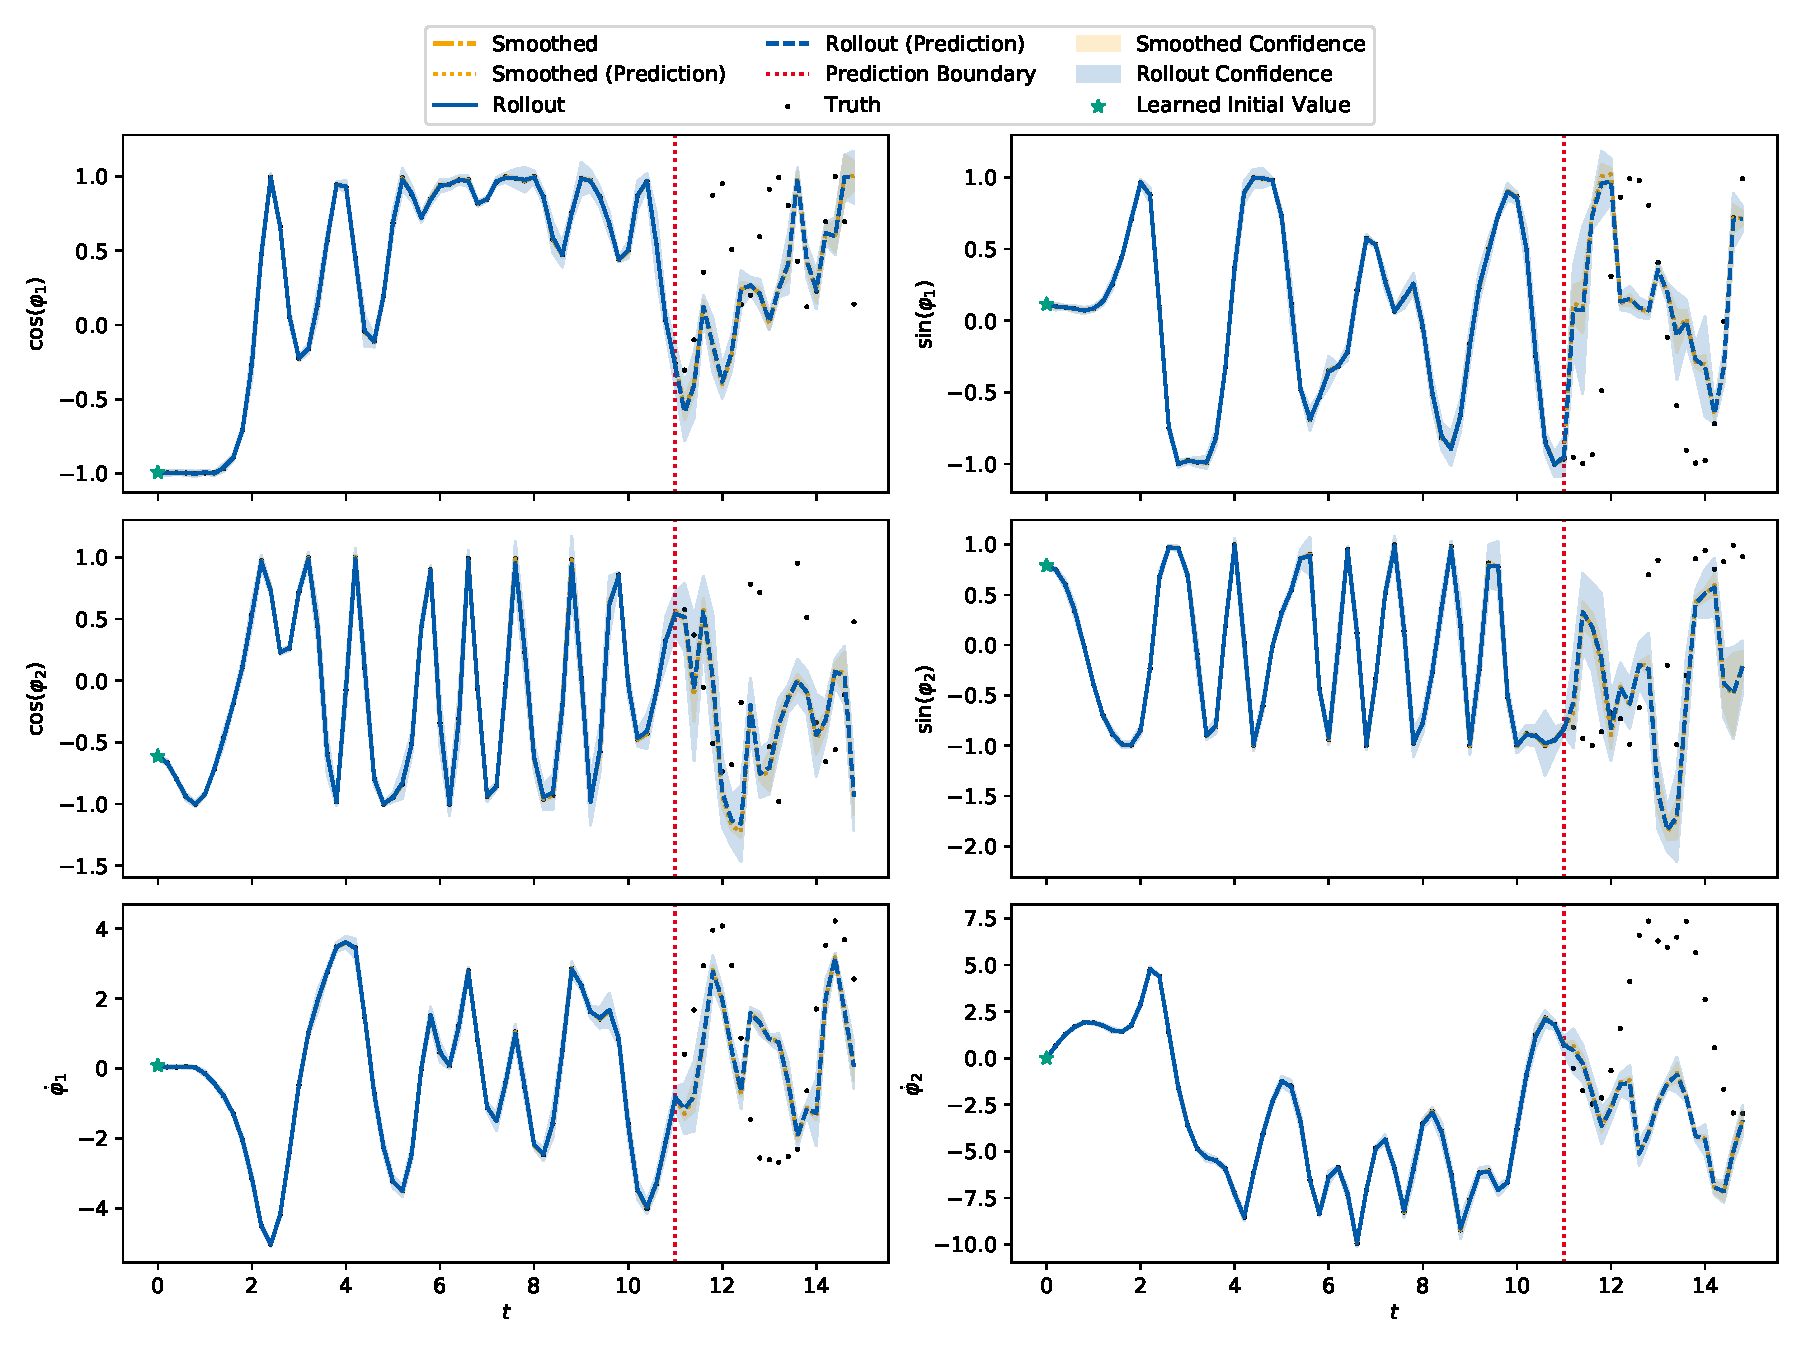
\includegraphics[width=\linewidth]{figures/results/cpu-vs-gpu/acrobot-gpu/rollout-observations-N0.pdf}
		\caption{Rollout of the double pendulum experiment that ran on the \ac{cpu}.}
		\label{fig:cpuVsGpuCpu}
	\end{figure}
	\begin{figure}
		\centering
		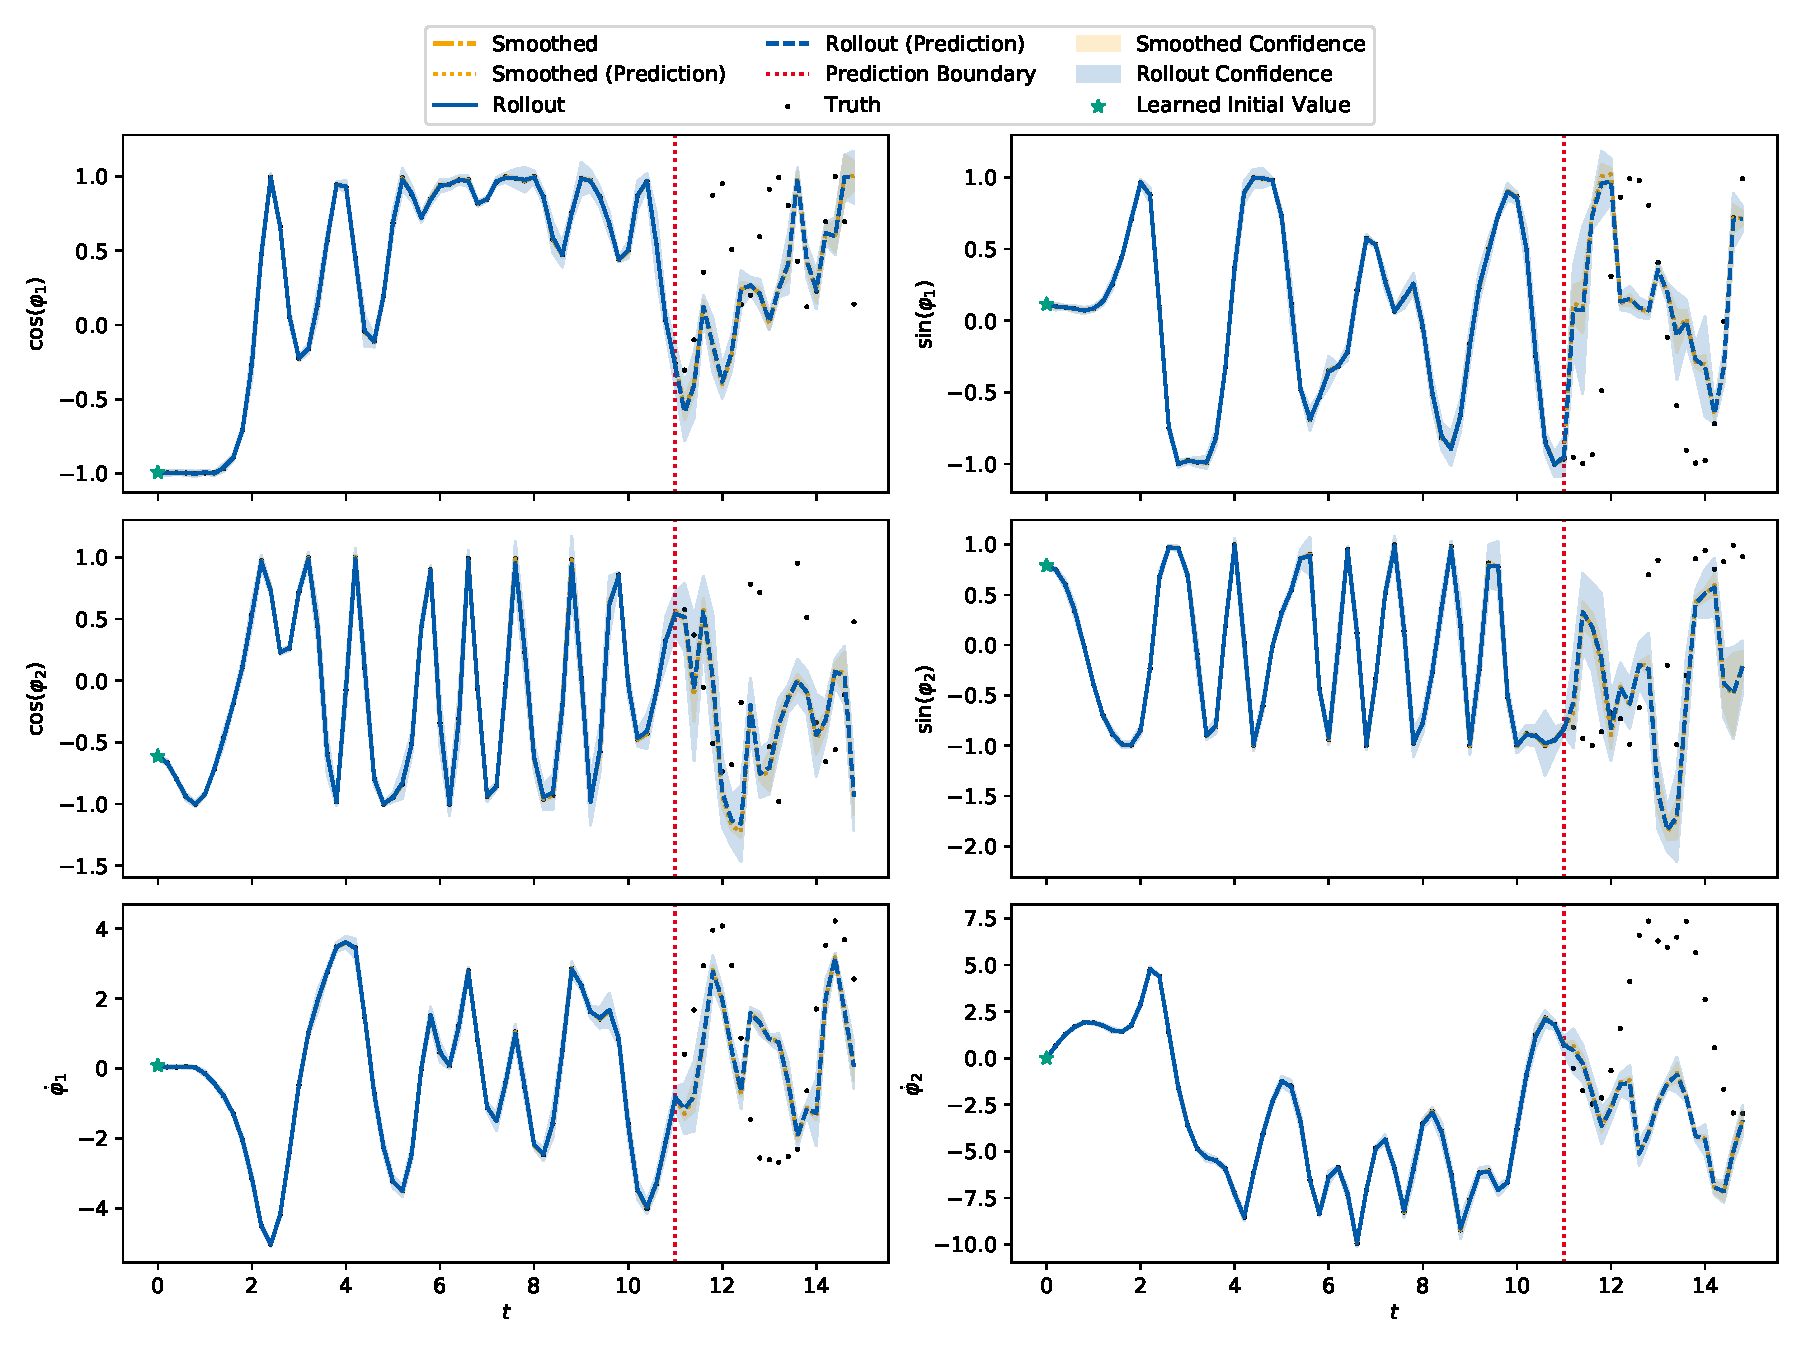
\includegraphics[width=\linewidth]{figures/results/cpu-vs-gpu/acrobot-gpu/rollout-observations-N0.pdf}
		\caption{Rollout of the double pendulum experiment that ran on the \ac{gpu}.}
		\label{fig:cpuVsGpuGpu}
	\end{figure}
% end

\section{Plots for Single- and Multi-Sequence Learning}
	\label{app:plotsSingleMulti}

	Plot overview:
	\begin{itemize}
		\item Damped pendulum experiment on a single observation sequence:~\autoref{fig:plotsSingleSequence}
		\item Damped pendulum experiment on a multiple (two) observation sequence:~\autoref{fig:plotsMultiSequence}
	\end{itemize}

	\begin{figure}
		\centering
		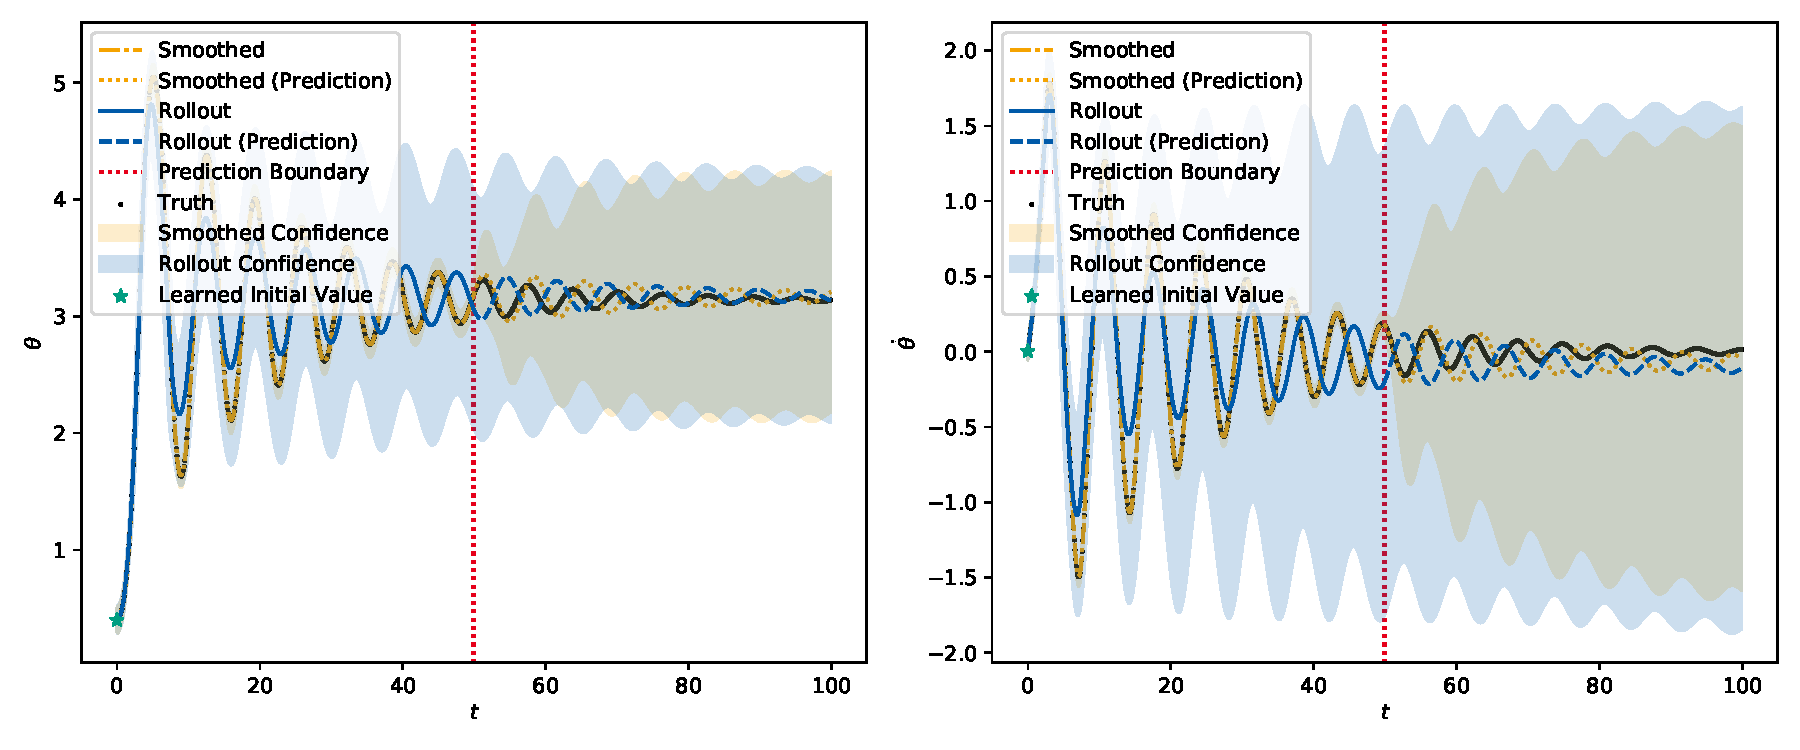
\includegraphics[width=\linewidth]{figures/results/single-vs-multi-sequence/pendulum-damped-single/rollout-observations-N0.pdf}
		\caption{Rollout of the damped pendulum experiment learning on a single observation sequence.}
		\label{fig:plotsSingleSequence}
	\end{figure}
	\begin{figure}
		\centering
		\begin{subfigure}{\linewidth}
			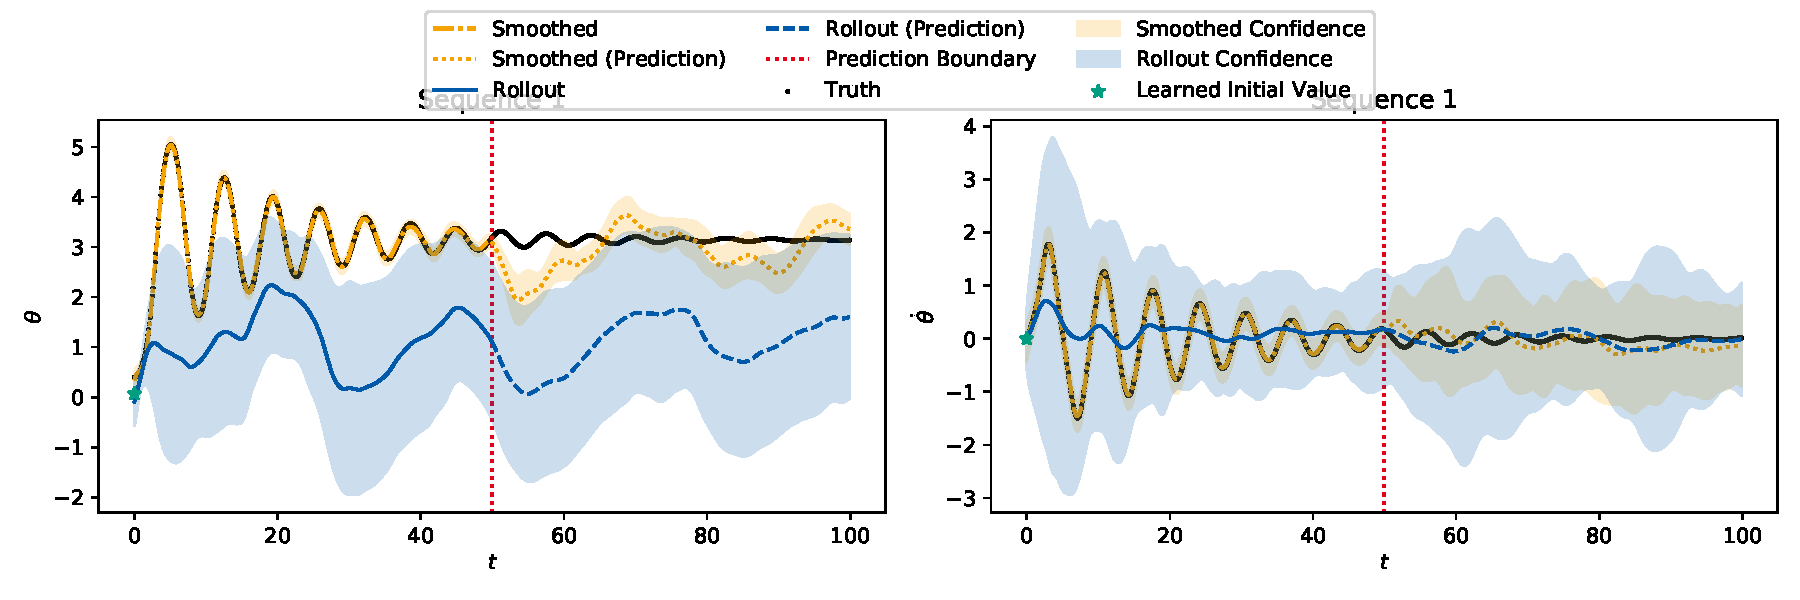
\includegraphics[width=\linewidth]{figures/results/single-vs-multi-sequence/pendulum-damped-multi/rollout-observations-N0.pdf}
		\end{subfigure} \\
		\begin{subfigure}{\linewidth}
			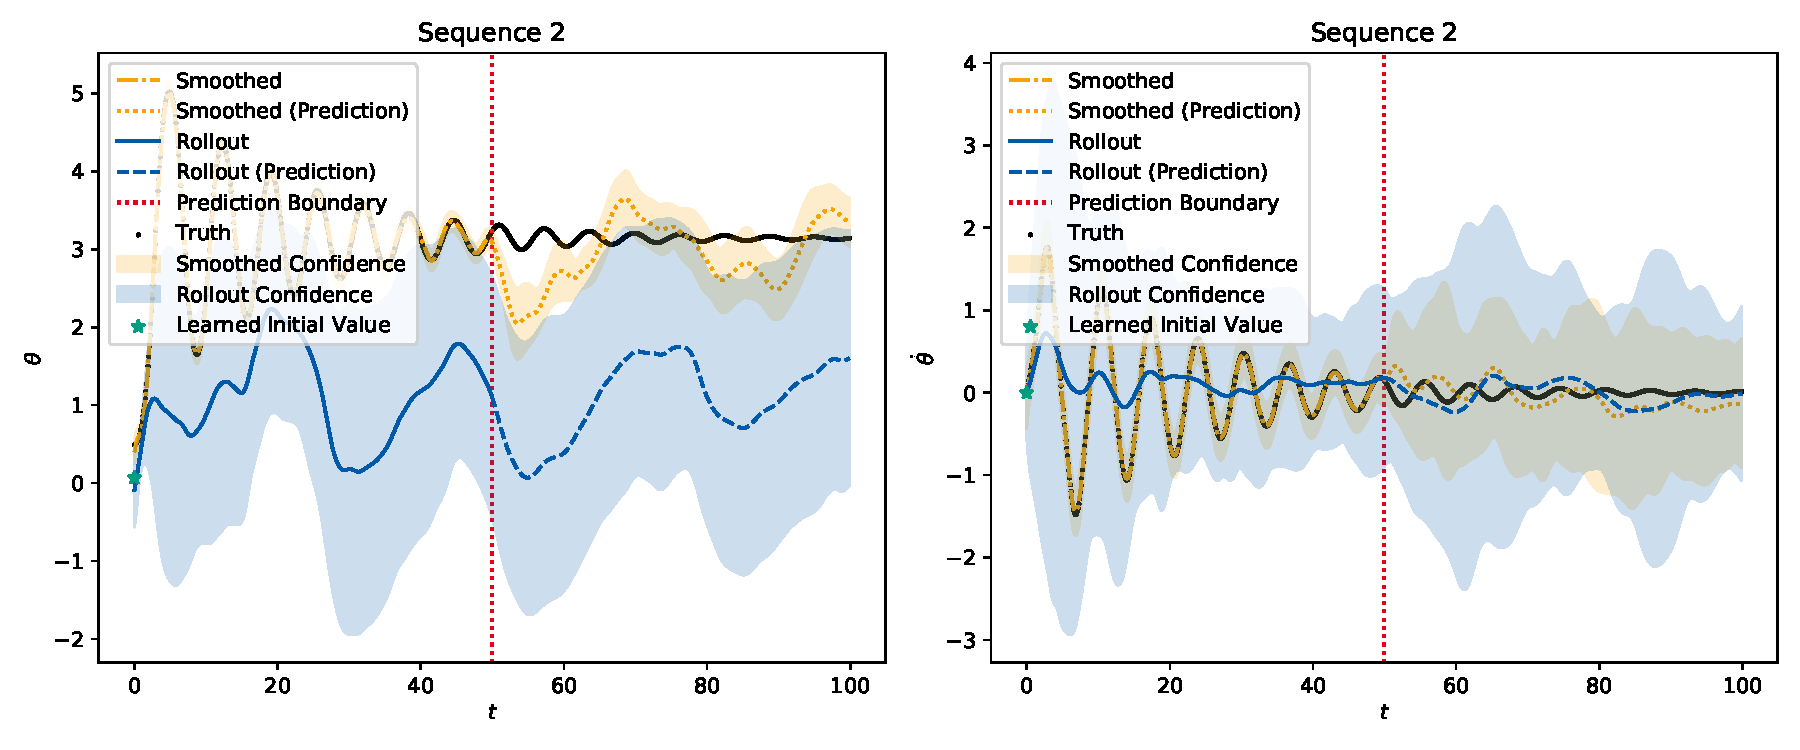
\includegraphics[width=\linewidth]{figures/results/single-vs-multi-sequence/pendulum-damped-multi/rollout-observations-N1.pdf}
		\end{subfigure}
		\caption{Rollout of the damped pendulum experiment learning on multiple (two) observation sequences. The top row is the first observation sequence, the bottom row is the second observation sequence.}
		\label{fig:plotsMultiSequence}
	\end{figure}
% end

\section{Remaining Plots}
	\label{app:remainingPlots}

	Plot overview:
	\begin{itemize}
		\item Gym cartpole, 1-dimensional latent, rollout with confidence:~\autoref{fig:cartpoleRolloutL02Appendix}
		\item Gym cartpole, 10-dimensional latent, rollout without confidence:~\autoref{fig:cartpoleRolloutL10Appendix}
		\item Gym cartpole, 31-dimensional latent, rollout without confidence:~\autoref{fig:cartpoleRolloutL14Appendix}
	\end{itemize}

	\begin{figure}
		\centering
		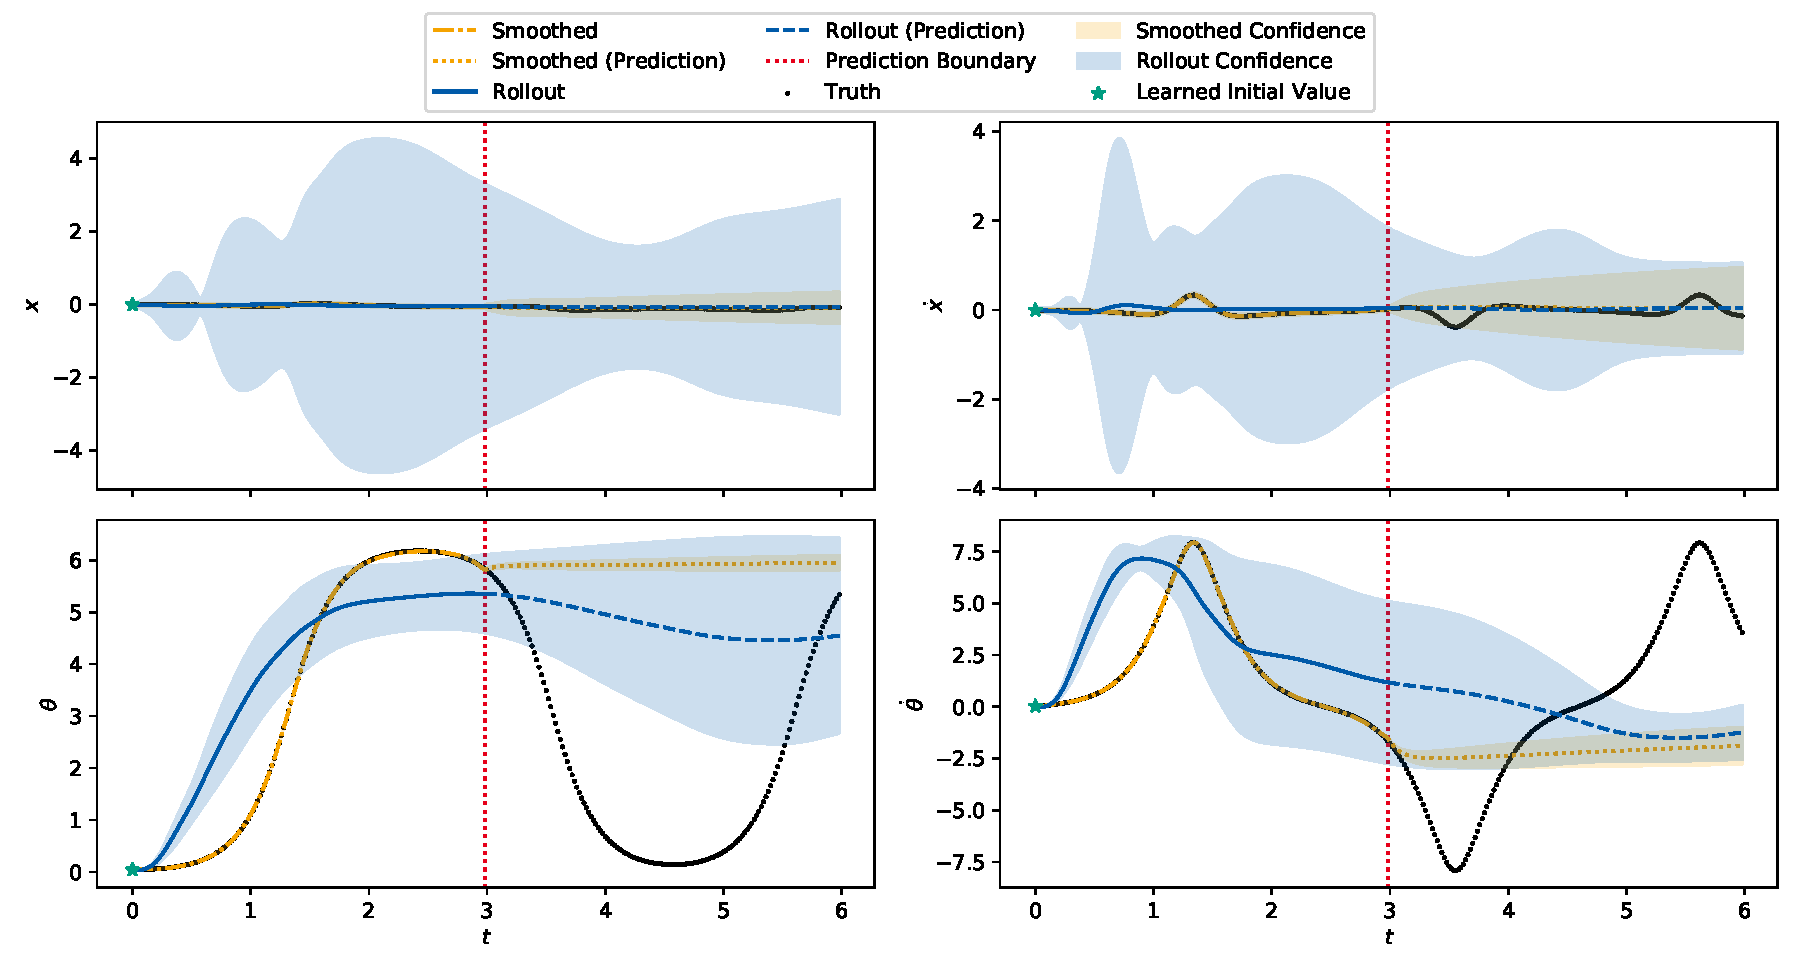
\includegraphics[width=\linewidth]{figures/results/cartpole-gym/run-latent-dim-02/rollout-observations-N0.pdf}
		\caption{This plot shows the same data as in~\autoref{fig:cartpoleRolloutL02}, but with the confidence shown. As the confidence is quite low, this plot is hard to interpret which is the reason why we removed the confidence plot in the first place.}
		\label{fig:cartpoleRolloutL02Appendix}
	\end{figure}

	\begin{figure}
		\centering
		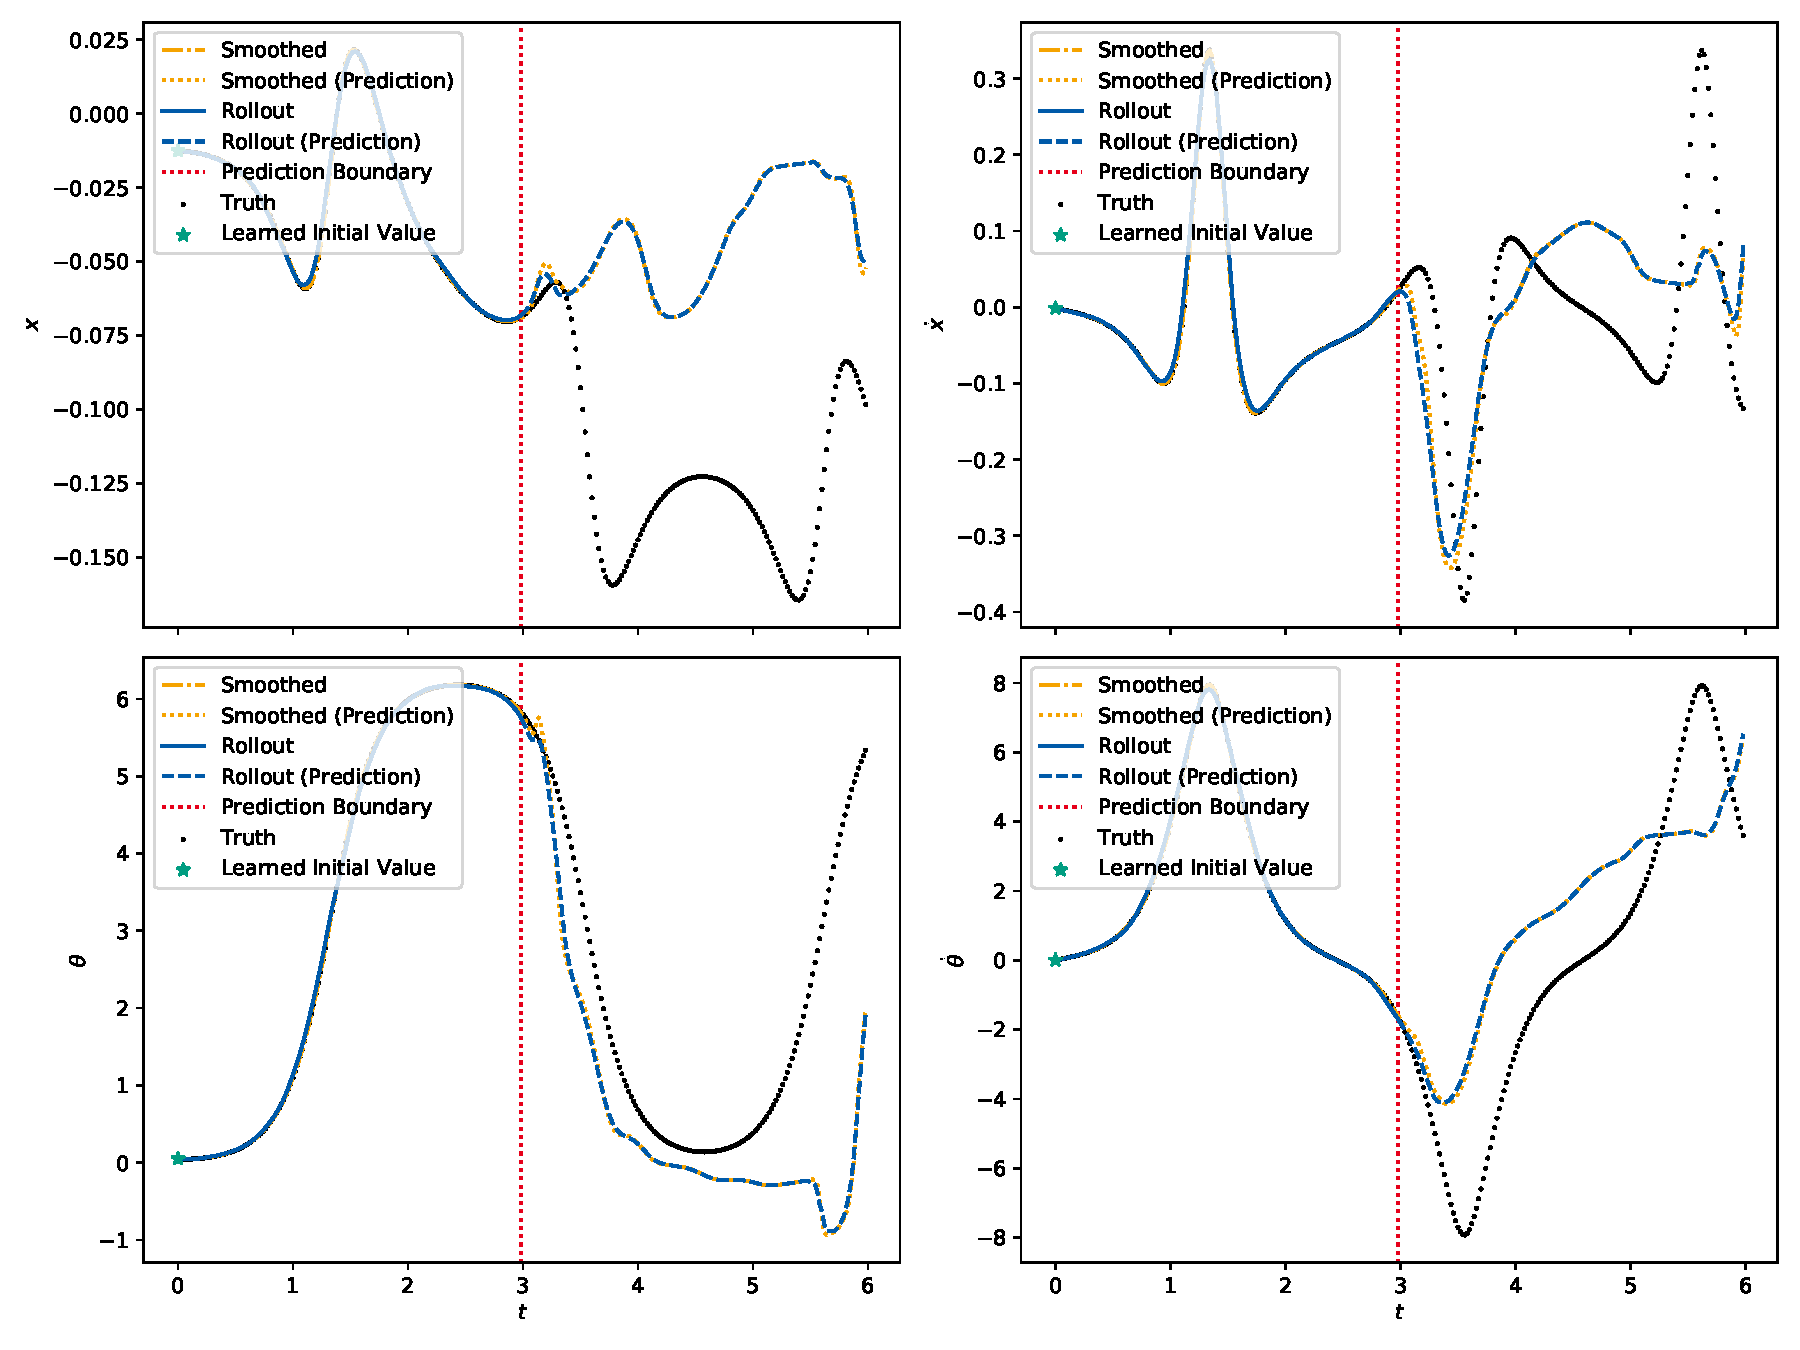
\includegraphics[width=\linewidth]{figures/results/cartpole-gym/run-latent-dim-10/without-confidence/rollout-observations-N0.pdf}
		\caption{This plot shows the same data as in~\autoref{fig:cartpoleRolloutL10}, but without the confidence shown.}
		\label{fig:cartpoleRolloutL10Appendix}
	\end{figure}

	\begin{figure}
		\centering
		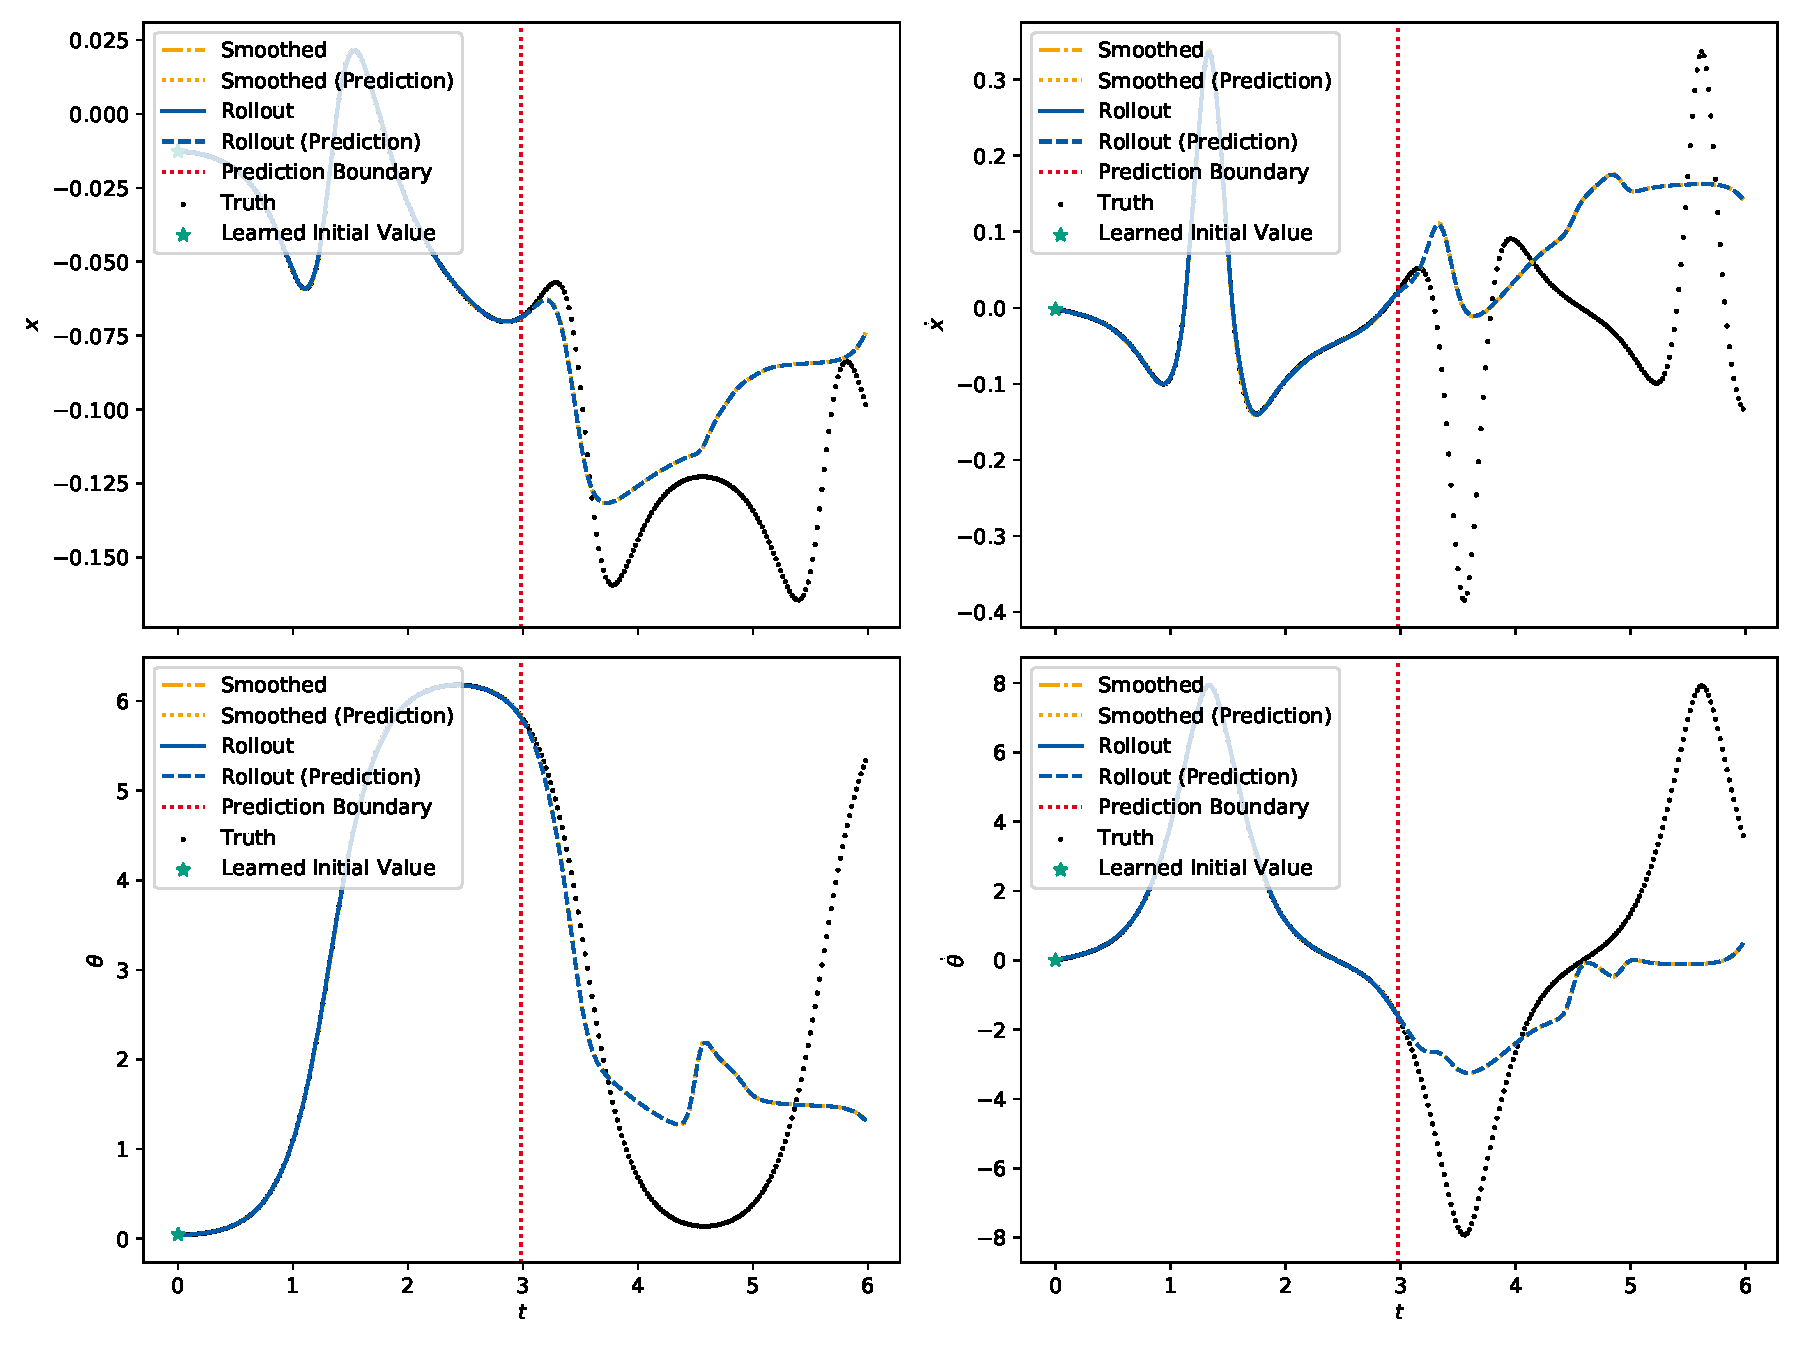
\includegraphics[width=\linewidth]{figures/results/cartpole-gym/run-latent-dim-16/without-confidence/rollout-observations-N0.pdf}
		\caption{This plot shows the same data as in~\autoref{fig:cartpoleRolloutL16}, but without the confidence shown.}
		\label{fig:cartpoleRolloutL16Appendix}
	\end{figure}
% end
